\subsection{2.1 Elektrisches Feld}
    \begin{tabular}{l|l l}
        Homogenes Feld & Inhomogenes Feld & 
        \\(Plattenkondensator) & (Punktladung) & 
        \\
        \\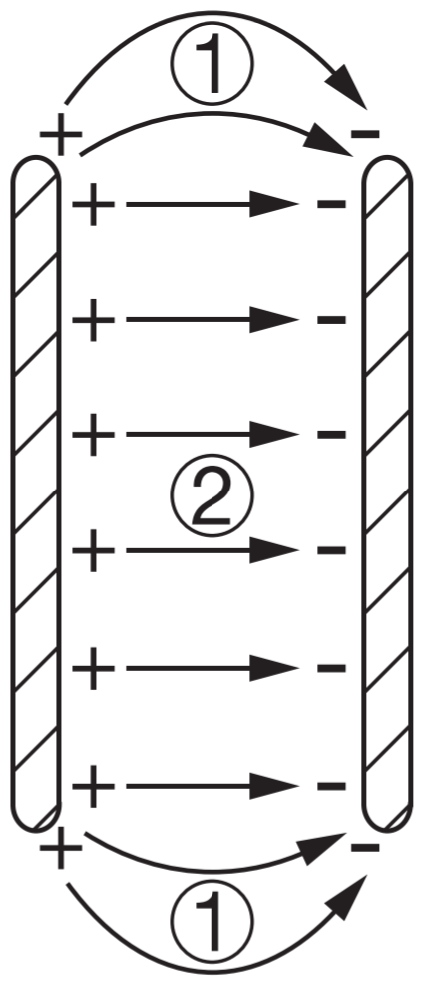
\includegraphics[width = 10mm]{src/images/kondensator.png} & 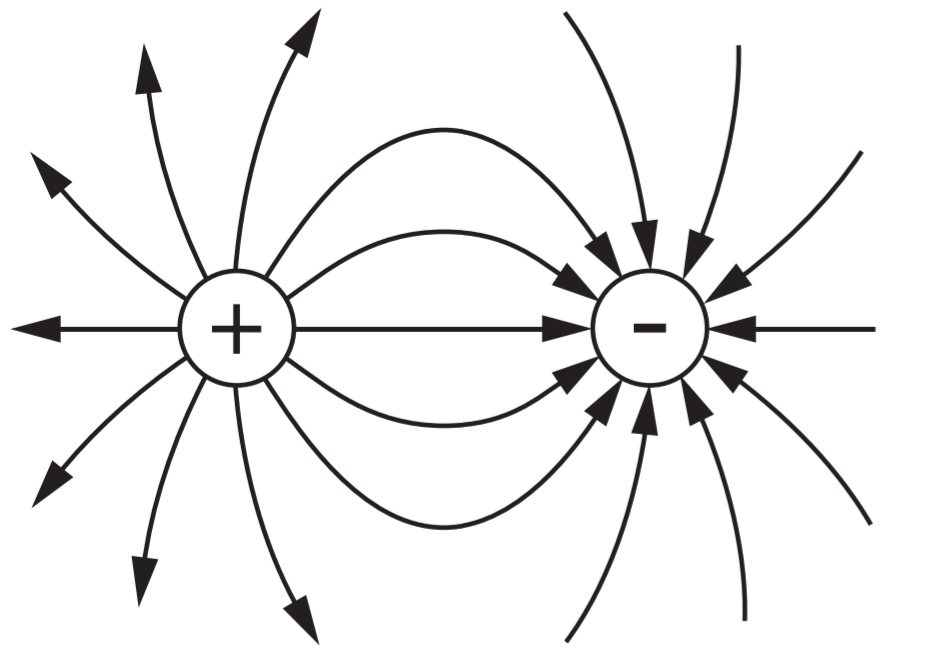
\includegraphics[width = 21mm]{src/images/zwei_punktladung.png} & 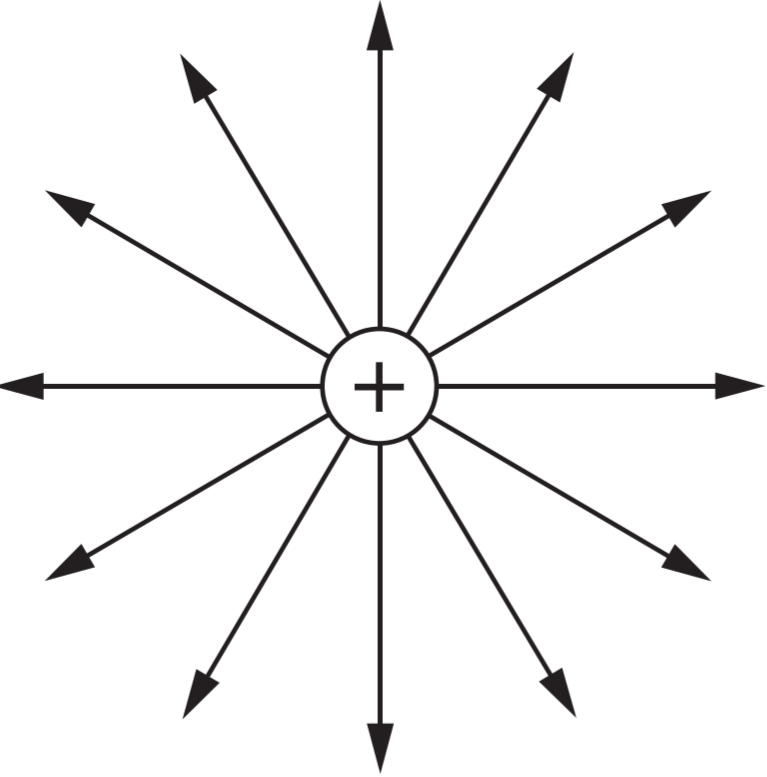
\includegraphics[width = 15mm]{src/images/punktladung.png}
    \end{tabular}
    \vspace{2mm}

    Quick facts:
    \begin{itemize}
        \item Jede Ladung erzeugt ein $E$ - Feld \vspace{-1mm}
        \item Feldlinien von + nach - \vspace{-1mm}
        \item Feldlinien immer $\bot$ auf leitfähigen Körpern \vspace{-1mm}
        \item Feldlinien schneiden sich nie \vspace{-1mm}
        \item Innerhalb von Leitern gibt es kein Feld
    \end{itemize}

